\documentclass[12pt]{article}
\usepackage{graphicx}
\usepackage{float}
\begin{document}
\title{Statistics 12, Lab 2}
\date{February 5th, 2019}
\author{Michael Wu\\UID: 404751542}
\maketitle

\section*{Exercise 1}

\paragraph{a)}

I loaded the data with the following code.
\begin{verbatim}
flint <- read.csv("flint.csv")
\end{verbatim}

\paragraph{b)}

I ran the following code.
\begin{verbatim}
mean(flint$Pb >= 15)
\end{verbatim}
This output that 4.436229\% of locations tested had dangerous lead levels.

\paragraph{c)}

I ran the following code.
\begin{verbatim}
mean(flint$Cu[flint$Region == "North"])
\end{verbatim}
This output that the mean copper level for test sites in the North region
was 44.6424 parts per billion.

\paragraph{d)}

I ran the following code.
\begin{verbatim}
mean(flint$Cu[flint$Pb >= 15])
\end{verbatim}
This output that the mean copper level for test sites with dangerous lead levels
was 305.8333 parts per billion.

\paragraph{e)}

I ran the following code.
\begin{verbatim}
mean(0 < flint$Pb & flint$Pb < 15)
\end{verbatim}
This output that 40.11091\% of locations tested had lead levels above zero parts per
billion and below the dangerous threshold.

\paragraph{f)}

I ran the following code.
\begin{verbatim}
mean(flint$Pb)
mean(flint$Cu)
\end{verbatim}
This output that the mean lead level was 3.383272 parts per billion and the mean copper
level was 54.58102 parts per billion.

\paragraph{g)}

I ran the following code.
\scriptsize
\begin{verbatim}
boxplot(flint$Pb, main="Lead Levels in Flint Water",
        xlab="Water Samples from Houses", ylab="Lead (Parts per Billion)")
\end{verbatim}
\normalsize
This generated the following plot.
\begin{figure}[H]
    \begin{center}
        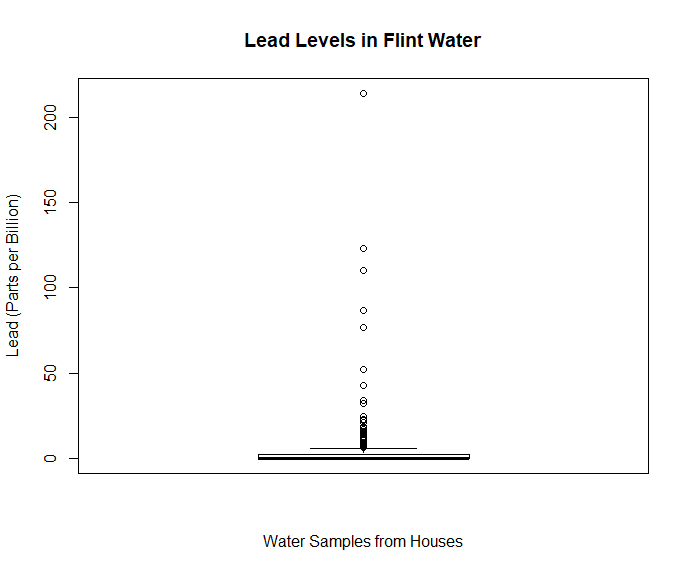
\includegraphics[width=4.5in]{exercise1g.png}
    \end{center}
\end{figure}

\paragraph{h)}

The mean does not seem to be a good measure of center for the data, as it is heavily right skewed.
A more useful statistic is the median which is zero parts per billion. Alternatively, another
analysis could be run with the log of the lead levels, as this may produce more interpretable results.

\section*{Exercise 2}

\paragraph{a)}

I ran the following code.
\scriptsize
\begin{verbatim}
plot(life$Life~life$Income, col="blue", cex = 0.5, pch = 19,
     xlab = "Income per Capita ($)", ylab = "Life Expectancy (Years)",
     main = "Income vs Life Expectancy")
\end{verbatim}
\normalsize
This generated the following plot.
\begin{figure}[H]
    \begin{center}
        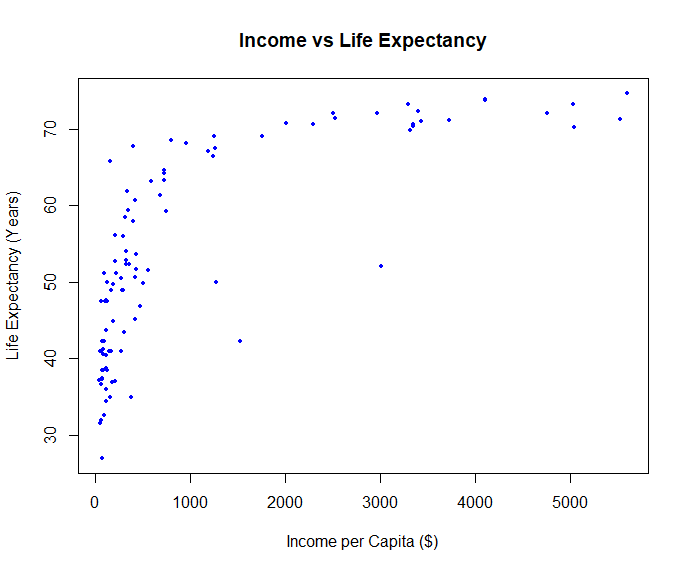
\includegraphics[width=4.5in]{exercise2a.png}
    \end{center}
\end{figure}
It seems that income has a strong positive correlation with life expectancy until around \$1000
income per capita. Then any additional income per capita does not seem to increase life expectancy
much past 70 years.

\paragraph{b)}

I ran the following code.
\begin{verbatim}
boxplot(life$Income, main="Income Boxplot",
        xlab="Income per Capita by Country", ylab="Amount ($)")
histogram(life$Income, main="Income Histogram",
          xlab="Income per Capita by Country ($)")
\end{verbatim}
This generated the following plots.
\begin{figure}[H]
    \begin{center}
        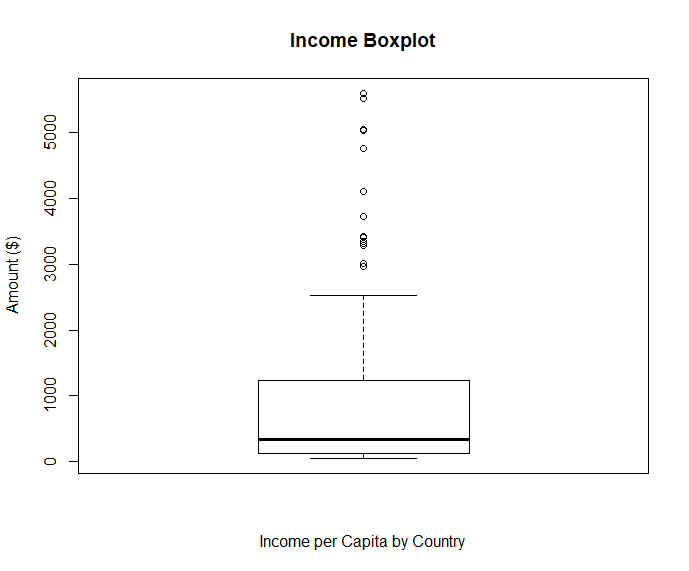
\includegraphics[width=2.5in]{exercise2b-box.png}
        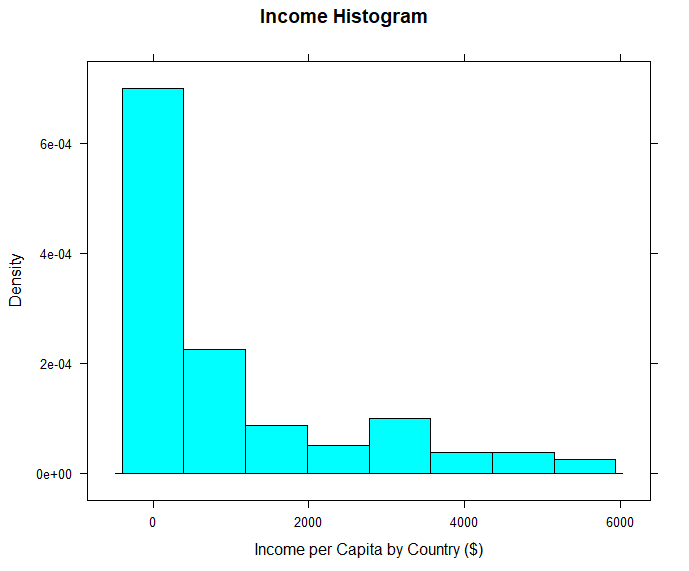
\includegraphics[width=2.5in]{exercise2b-histogram.png}
    \end{center}
\end{figure}
Yes it seems like there are outliers. Most countries have an income per capita of less than \$2000.
So the most wealthy countries are outliers.

\paragraph{c)}

I ran the following code.
\begin{verbatim}
incomeBelow1000 <- life[life$Income < 1000, ]
incomeAtLeast1000 <- life[life$Income >= 1000, ]
\end{verbatim}

\paragraph{d)}

I ran the following code.
\scriptsize
\begin{verbatim}
plot(incomeBelow1000$Life~incomeBelow1000$Income, col="blue", cex = 0.5, pch = 19,
     xlab = "Income per Capita ($)", ylab = "Life Expectancy (Years)",
     main = "Income vs Life Expectancy for Income Below $1000")
cor(incomeBelow1000$Income, incomeBelow1000$Life)
\end{verbatim}
\normalsize
This generated the following plot.
\begin{figure}[H]
    \begin{center}
        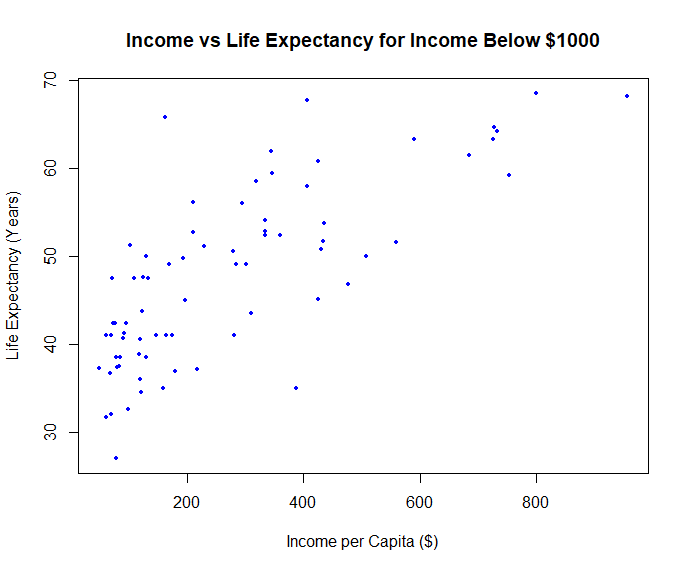
\includegraphics[width=4.5in]{exercise2d.png}
    \end{center}
\end{figure}
The correlation coefficient between life expectancy and income for this data was 0.752886.

\section*{Exercise 3}

\paragraph{a)}

I ran the following code.
\begin{verbatim}
summary(maas$lead)
summary(maas$zinc)
\end{verbatim}
It printed out the following summary statistics for lead.
\begin{verbatim}
Min. 1st Qu.  Median    Mean 3rd Qu.    Max.
37.0    72.5   123.0   153.4   207.0   654.0
\end{verbatim}
It printed out the following summary statistics for zinc.
\begin{verbatim}
 Min. 1st Qu.  Median    Mean 3rd Qu.    Max.
113.0   198.0   326.0   469.7   674.5  1839.06
\end{verbatim}
The IQR for zinc is \(674.5-198=476.5\) parts per million.

\paragraph{b)}

I ran the following code.
\begin{verbatim}
histogram(maas$lead, main="Lead in Maas River Bank Soil",
          xlab="Lead Parts per Million")
histogram(log(maas$lead), main="Lead in Maas River Bank Soil",
          xlab="Log(Lead Parts per Million)")
\end{verbatim}
This generated the following plots.
\begin{figure}[H]
    \begin{center}
        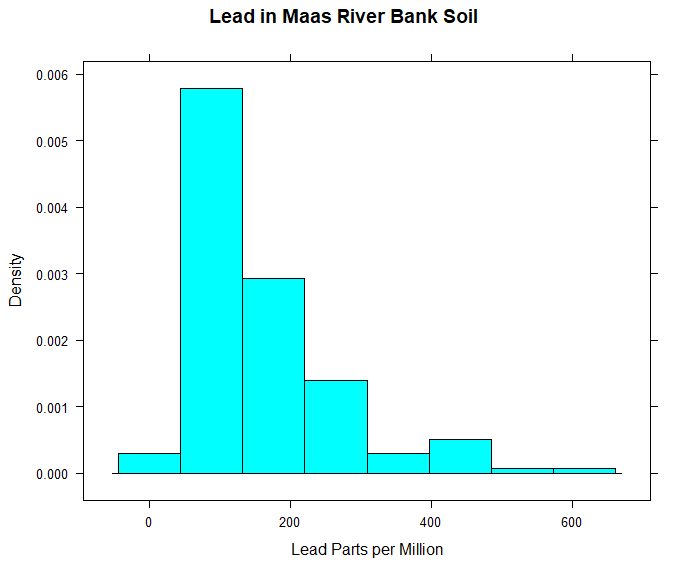
\includegraphics[width=2.5in]{exercise3b-normal.png}
        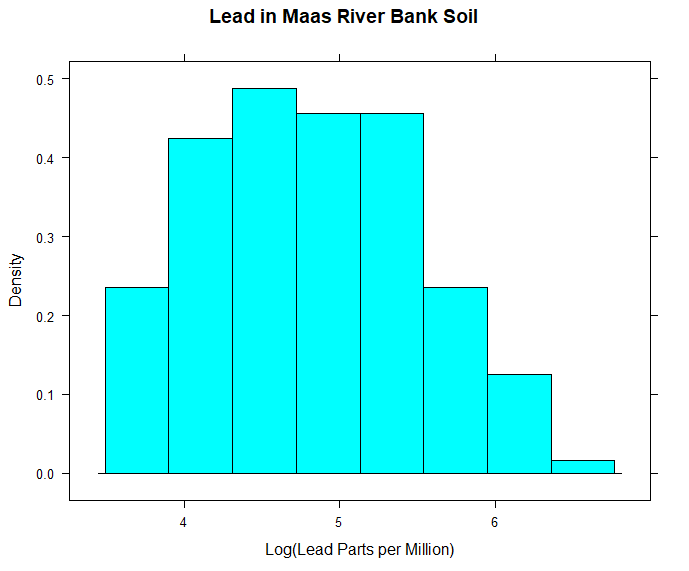
\includegraphics[width=2.5in]{exercise3b-log.png}
    \end{center}
\end{figure}

\paragraph{c)}

I ran the following code.
\scriptsize
\begin{verbatim}
plot(log(maas$lead)~log(maas$zinc), col="blue", cex = 0.5, pch = 19,
     xlab = "Log(Zinc Parts per Million)", ylab = "Log(Lead Parts per Million)",
     main = "Lead vs Zinc in Maas River Bank Soil")
\end{verbatim}
\normalsize
This generated the following plot.
\begin{figure}[H]
    \begin{center}
        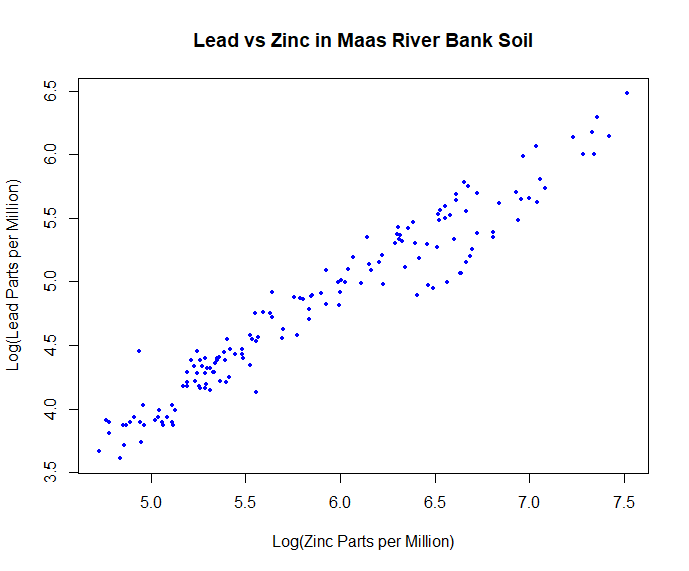
\includegraphics[width=4.5in]{exercise3c.png}
    \end{center}
\end{figure}
It appears that there is a strong, positive, linear correlation between the amount of lead and
the amount of copper found.

\paragraph{d)}

I ran the following code.
\scriptsize
\begin{verbatim}
colors <- c("pink", "red", "darkred")
levels <- cut(maas$lead, c(0, 150, 400, 1000))
plot(maas$x,maas$y, xlab="x", ylab="y", main="Lead Concentration Map", "n")
points(maas$x,maas$y, cex=maas$lead/mean(maas$lead),
       col=colors[as.numeric(levels)], pch=19)
\end{verbatim}
\normalsize
This generated the following plot.
\begin{figure}[H]
    \begin{center}
        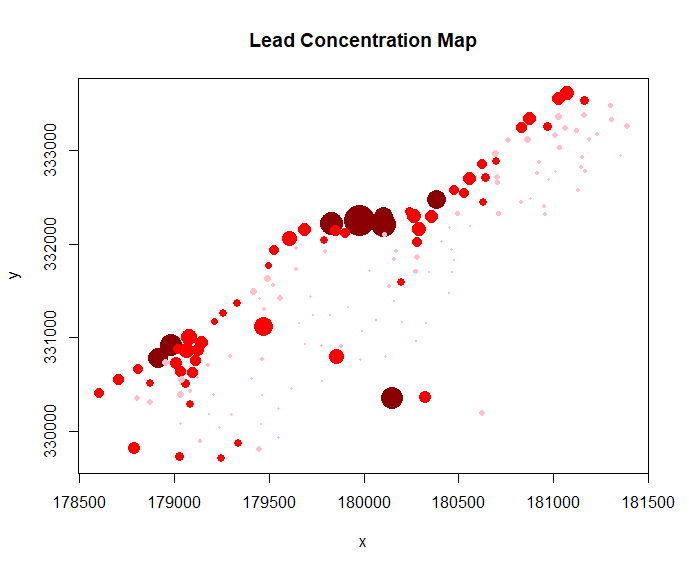
\includegraphics[width=4.5in]{exercise3d.png}
    \end{center}
\end{figure}

\section*{Exercise 4}

\paragraph{a)}

I ran the following code.
\scriptsize
\begin{verbatim}
plot(LA$Longitude,LA$Latitude, xlab="Longitude",
     ylab="Latitude", main="Los Angeles Neighborhood Centers", "n")
map("county", "California", add = TRUE)
points(LA$Longitude, LA$Latitude)
\end{verbatim}
\normalsize
This generated the following plot.
\begin{figure}[H]
    \begin{center}
        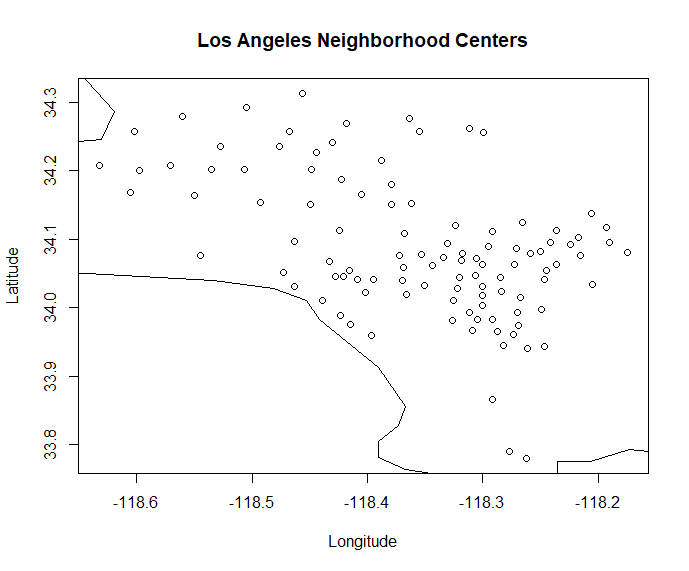
\includegraphics[width=4.5in]{exercise4a.png}
    \end{center}
\end{figure}

\paragraph{b)}

I ran the following code.
\scriptsize
\begin{verbatim}
LAFiltered <- LA[LA$Schools > 0, ]
plot(LAFiltered$Schools~LAFiltered$Income, col="blue", cex = 0.5, pch = 19,
     xlab = "Income ($)", ylab = "School Performance",
     main = "School Performance vs Income")
\end{verbatim}
\normalsize
This generated the following plot.
\begin{figure}[H]
    \begin{center}
        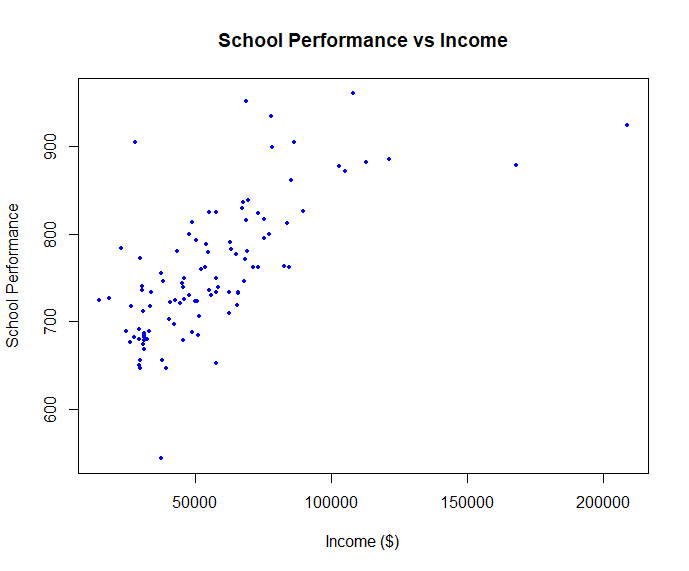
\includegraphics[width=4.5in]{exercise4b.png}
    \end{center}
\end{figure}
It seems that the income within a neighborhood is positively correlated with the school
performance in that neighborhood.

\paragraph{c)}

I ran the following code.
\begin{verbatim}
mean(LA$Income)
sd(LA$Income)
\end{verbatim}
The data has a mean income of \$58,129.05 and a standard deviation of \$30,976.76. Then the z-score of a new neighborhood
with an average income of \$100,000 is the following.
\[\frac{100000-58129.05}{30976.76}=1.3517\]
This z-score tells us that an income of \$100,000 is above average for a neighborhood, but not exceptionally above average.

\paragraph{d)}

I ran the following code.
\begin{verbatim}
mean(27152.29 < LA$Income & LA$Income < 89105.81)
mean(-3824.47 < LA$Income & LA$Income < 120082.57)
mean(-34801.23 < LA$Income & LA$Income < 151059.33)
\end{verbatim}
This indicated that 84.11215\% of neighborhoods had an income within one standard deviation from the mean,
96.26168\% of neighborhoods had an income within two standard deviations from the mean,
and 97.19626\% of neighborhoods had an income within three standard deviations from the mean. So my results
had a greater percentage within one standard deviation, a greater percentage within two standard deviations,
and a smaller percentage within three standard deviations than predicted by the empirical rule.
It does not match exactly because the data is skewed to the right.

\end{document}